\section{Entwurf}
\subsection{Komponentendiagramm}
Abbildung \ref{fig:Komponentendiagramm} auf Seite \pageref{fig:Komponentendiagramm} zeigt das Komponentendiagramm.

\begin{figure}[htp]
\centering
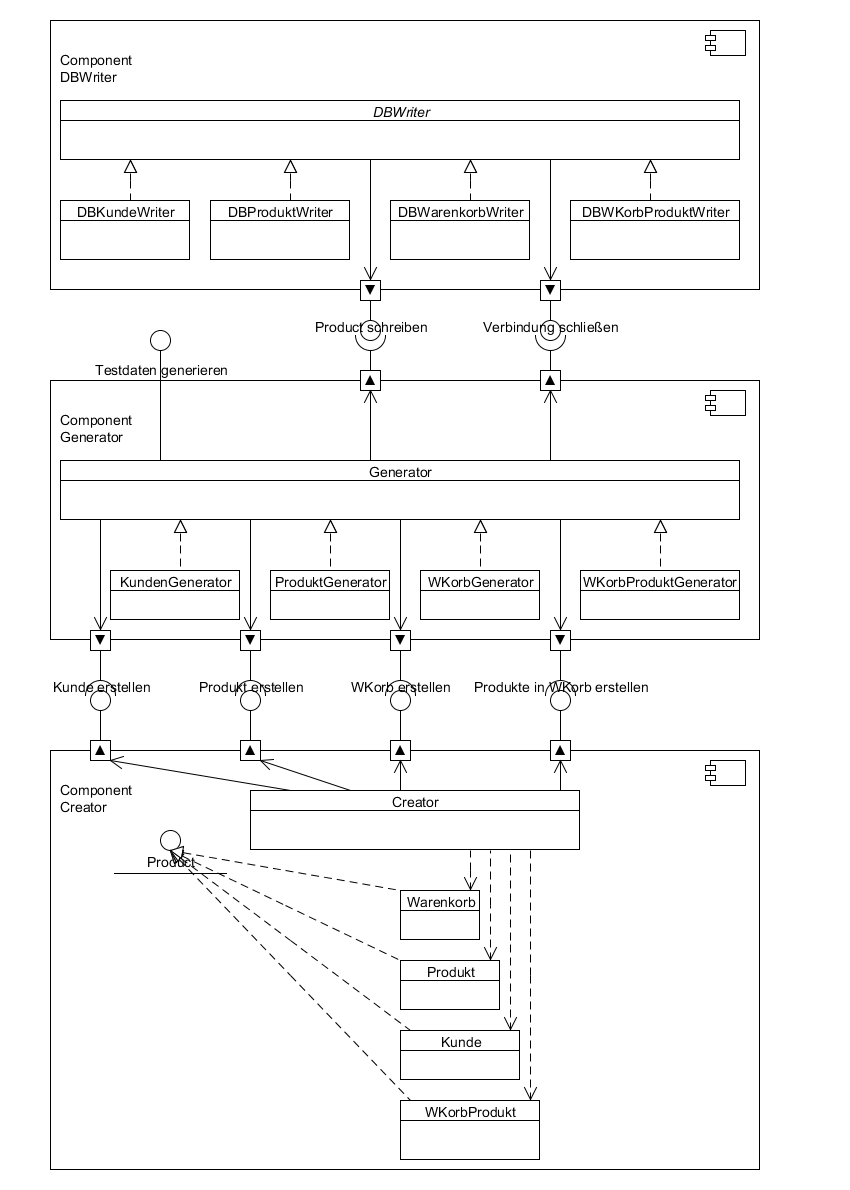
\includegraphics[width=0.8\textwidth]{Ingo/Bilder/Komponentendiagramm.png}
\caption{Komponentendiagramm}
\label{fig:Komponentendiagramm}
\end{figure}

\subsection{Entwurfsklassendiagramm der Generatorkomponente}
Abbildung \ref{fig:EntwurfGeneratorkomponente} auf Seite \pageref{fig:EntwurfGeneratorkomponente} zeigt das Entwurfsklassendiagramm der Generatorkomponente.

\begin{figure}[htp]
\centering
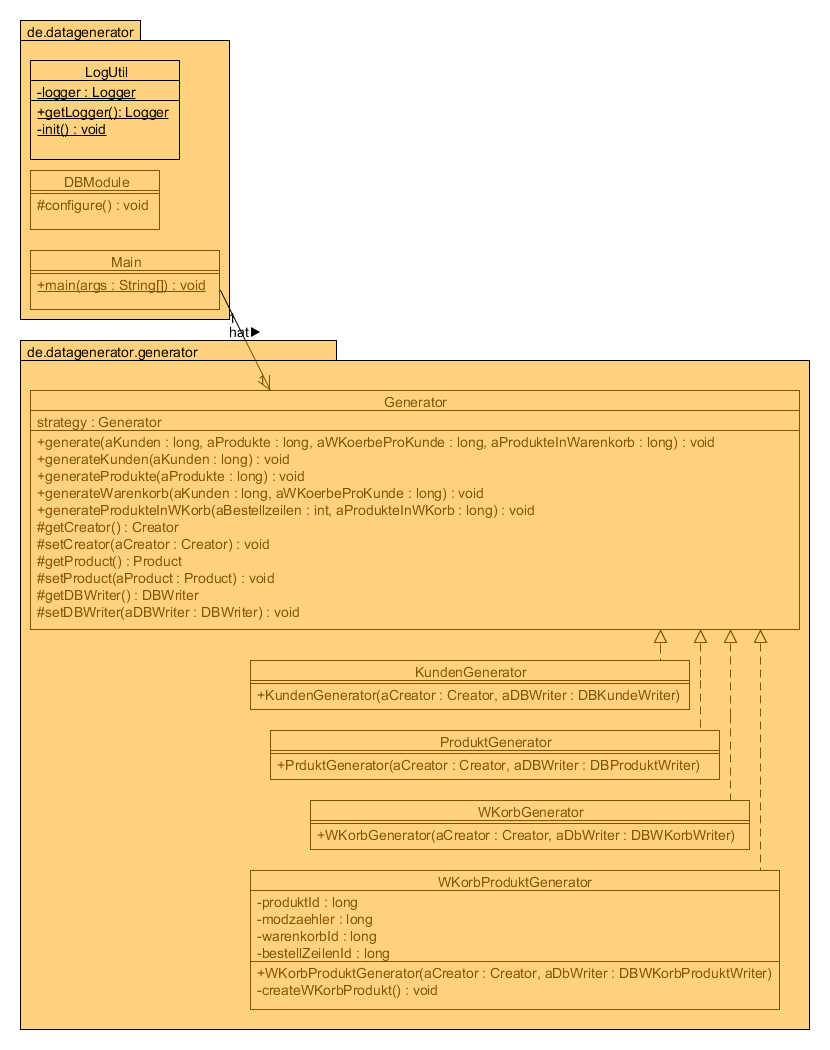
\includegraphics[width=0.8\textwidth]{Ingo/Bilder/EntwurfGeneratorkomponente.png}
\caption{Entwurf der Generatorkomponente}
\label{fig:EntwurfGeneratorkomponente}
\end{figure}

\subsection{Entwurfsklassendiagramm der DBWriterkomponente}
Abbildung \ref{fig:EntwurfDBWriterkomponente} auf Seite \pageref{fig:EntwurfDBWriterkomponente} zeigt das Entwurfsklassendiagramm der DBWriterkomponente.

\begin{figure}[htp]
\centering
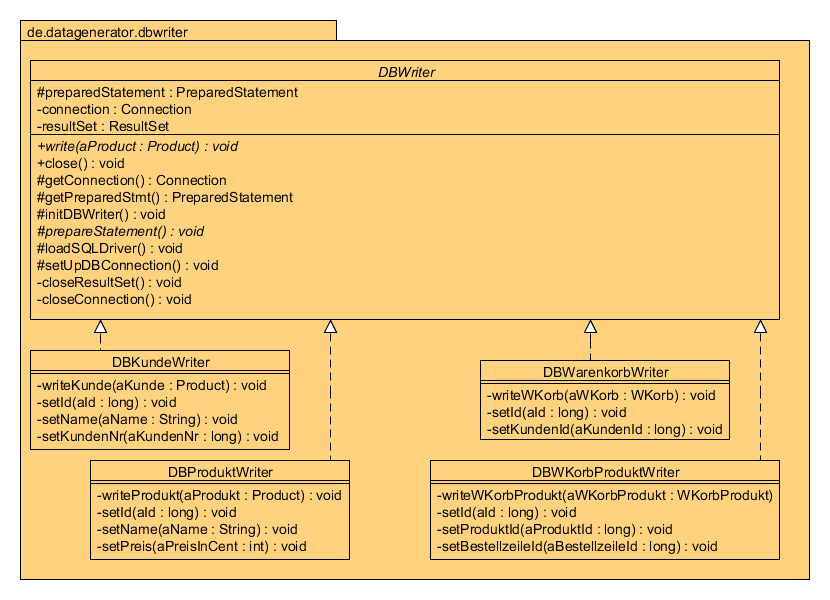
\includegraphics[width=0.8\textwidth]{Ingo/Bilder/EntwurfDBWriterkomponente.png}
\caption{Entwurf der DBWriterkomponente}
\label{fig:EntwurfDBWriterkomponente}
\end{figure}

\subsection{Entwurfsklassendiagramm der Creatorkomponente samt Datamodel}
Abbildung \ref{fig:EntwurfCreatorUndDatamodelKomponente} auf Seite \pageref{fig:EntwurfCreatorUndDatamodelKomponente} zeigt das Entwurfsklassendiagramm der Creatorkomponente und dem dazugeh�rigen Datamodel.

\begin{figure}[htp]
\centering
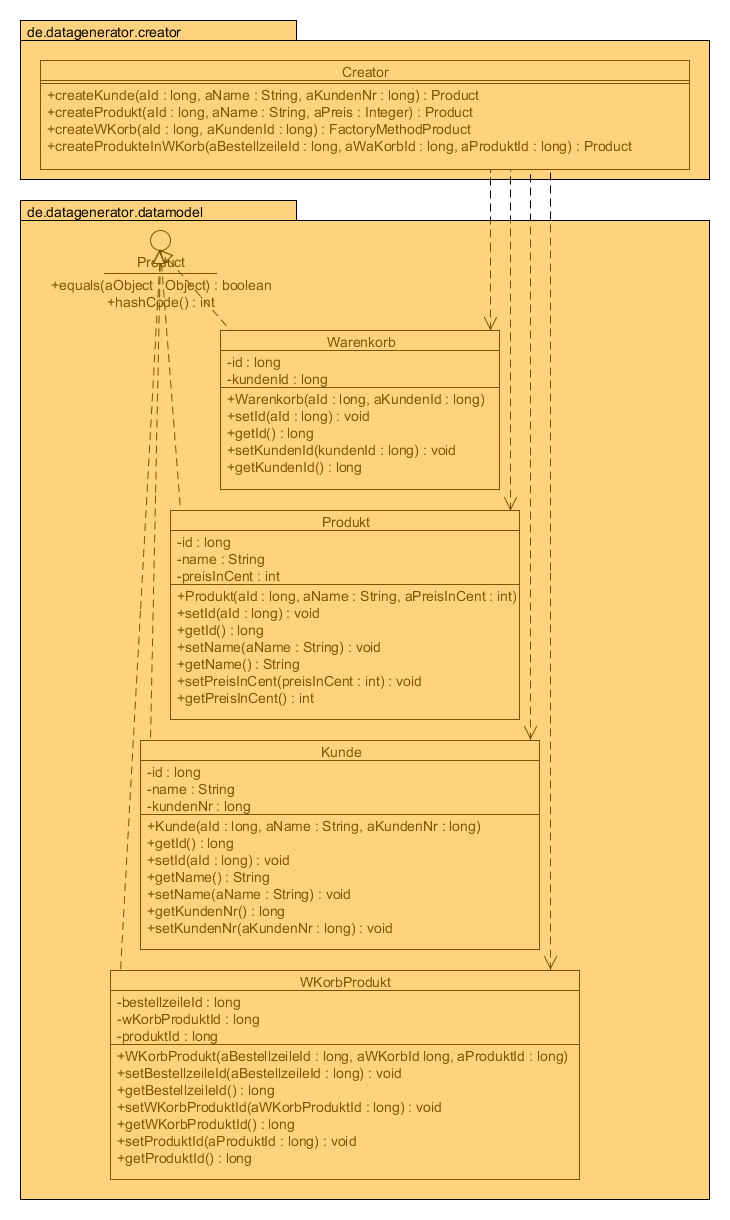
\includegraphics[width=0.8\textwidth]{Ingo/Bilder/EntwurfCreatorUndDatamodelKomponente.png}
\caption{Entwurf der Creatorkomponente}
\label{fig:EntwurfCreatorUndDatamodelKomponente}
\end{figure}

\subsection{Stored Procedures}
Client-Server-System als Zwei-Schichten-Architekur.

\subsection{Kontext und Dependency Injection mit Google Guice}
Architekurmuster

\subsection{Entwurfsmuster}